\documentclass{article}
\usepackage{graphicx} % Required for inserting images
\usepackage{CJKutf8}
\usepackage{amsthm}
\usepackage{mdframed}
\usepackage{float}

% 自定義 "Definition" 環境
\newmdtheoremenv{definition}{Definition}

\title{hw9}
\author{110201534 楊成偉}
\date{}

\begin{document}
\begin{CJK*}{UTF8}{bkai}
\maketitle

\section*{problem 1}
consider a path $P_{4}$, if we add edge 13 and 24,then we get a 2-connected graph(since if we remove vertex 2 and vertex 3 will make the graph disconnected), and consider the path $P_{4}$, we can not find another internally disjoint path since $P_{4}$ has already contain all vertice of the graph, so the statement in problem 1 is false.

\section*{problem 2}
\begin{figure}[H]
    \centering
    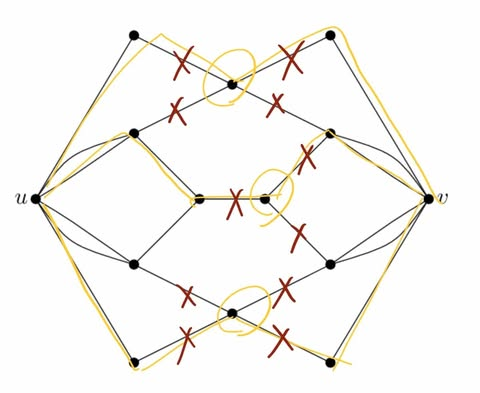
\includegraphics[scale = 0.3]{hw9.jpg}
    \caption{show how to choose the cut-vertex}
\end{figure}
In the diagram above, we demonstrate that removing three vertices (yellow circles) along with their connected edges (red crosses) will result in there is no \( u \)-\( v \) paths in G - S, where S consist of the 3 vertice.
so we can get the conclusion that $\kappa(u,v) = 3$
\section*{problem 3}
\subsection*{step1}
Given an X,Y-bigraph G, construct G' by adding vertices x,y such that x is adjacent to all
vertices in X and y is adjacent to all vertices in Y.
\subsection*{step2}
it is obvious that $\lambda_{G'}(x , y) \leq \alpha'(G)$, let M be a matching such that size of M is $\alpha'(G)$, and for each u-v edge in M, we can construct a x-y path ({x, u, v, y}), then we have $\lambda_{G'}(x , y) = \alpha'(G)$
\subsection*{step3}
Since \( G \) is a bipartite graph, for the vertices in the minimum vertex cover of \( G \), the vertices they are connected to must belong to the other part of the bipartite graph. Therefore, if we remove all the vertices in the vertex cover, the bipartite graph will become disconnected.
then we can get the $\kappa_{G'}(x,y) = \beta(G)$
\subsection*{step4}
By conclusion in step2, we have $\lambda_{G'}(x , y) = \alpha'(G)$, Suppose there is a set of pairwise internally disjoint \(x, y\)-paths such that the size of this set equals \( \lambda_{G'}(x, y) \). If we remove one vertex from each path (forming the set \(S\)), then there will be no \(x, y\)-paths in \(G' - S\). This allows us to conclude that \( \kappa(G) = \alpha'(G) \).

and it is obvious that $\kappa_{G'}(x,y) = \kappa(G)$ so we finish this proof.
\end{CJK*}
\end{document}
